\documentclass{beamer}
\usepackage{amsmath}
\usepackage{graphicx}

%% ===========================================
%% ===========================================
\title{\huge Martrix Project}
\author{Gunasekhar and Dileep Chandra}
\institute{IITH}
\date{\today}

%% ===========================================

%% ===========================================
\begin{document}


\begin{frame}[plain]
    \titlepage
\end{frame}
%% ===========================================
%% ===========================================

\section{First Section}
\subsection{Subsection Example}

%% ===========================================
%% ===========================================
%	PRESENTATION SLIDES
%% ===========================================
%% ===========================================

%% ===========================================
%% ===========================================

\begin{frame}
\frametitle{Question:14}
A line drawn through the point p=(4,7)
cuts the circle $X^2+Y^2=9$at the points A and B.Find PA.PB.
\end{frame}

%% ===========================================
%% ===========================================

\begin{frame}
\frametitle{Matrix Transformation}
\begin{itemize}
\item Circle equation:$X^TX=9$
\item Matrix form of a line through a given point P:
    X=P+m$\lambda$
\item i.e;
X=\begin{bmatrix}
    4\\
    7
\end{bmatrix}+$m\lambda$    
\item Let the line through given point cut the circle at the points A,B.
\item $A^TA=9$ and $B^TB=9$\\
A=P+m$\lambda_1$ and B=P+m$\lambda_2$
\item So,\\
$(p+m\lambda)^T(P+m\lambda)=9$ is a quadratic equation in $\lambda$ with roots $\lambda_1$ and $\lambda_2$.
\item On expanding\\
$||m||\lambda^2+2P^Tm\lambda+||P||^2-9=0$
\end{itemize}
\end{frame}
\begin{frame}
\frametitle{Condition for line to intersect the circle}
\begin{itemize}
\item the roots of the quadratic equation are\\
$\lambda_1=-P^T+\sqrt{(P^Tm)^2+9-||P||^2}$ and\\
$\lambda_2=-P^T-\sqrt{(P^Tm)^2+9-||P||^2}$
\item condition for line to intersect the circle:\\
$(P^Tm)^2>=||P||^2-9$\\
$(P^Tm)^2>=56$
\end{itemize}
\end{frame}
%% ===========================================
%% ===========================================
\begin{frame}
\frametitle{Figure}
\begin{figure}[htp]
\centering
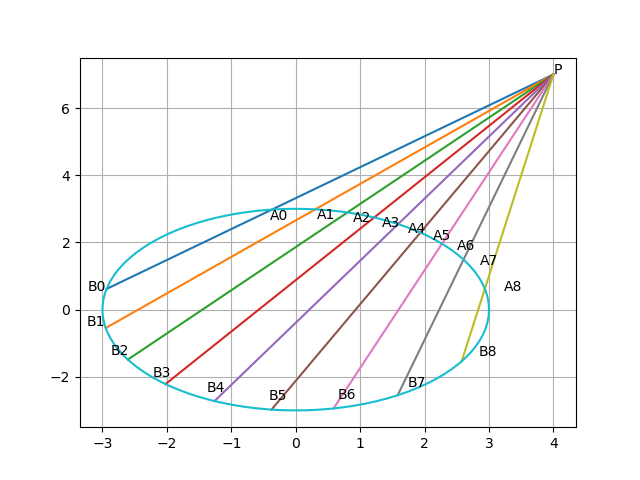
\includegraphics[width=5cm,height=8cm]{Figure}
\caption{graph}
\label{fig:graph}
\end{figure}
\end{frame}
\begin{frame}
\frametitle{Solution}
\begin{itemize}
\item $PA.PB=||P-A||.||P-B||$\\
$PA.PB=||m\lambda_1||.||m\lambda_2||=\lambda_1\lambda_2||m||^2$
\item Obtained quadratic equation\\
$||m||\lambda^2+2P^Tm\lambda+||P||^2-9=0$
\item Product of roots:\\
$\lambda_1\lambda_2=\frac{||P||^2-9}{||m||^2}$
\item rearranging the equation\\
PA.PB=$|(||P||^2-1)|$
\item PA.PB=(65-9)=56
\end{itemize}
\end{frame}

\begin{frame}
\frametitle{Conclusion}
\begin{itemize}
\item PA.PB=56=Constant
\item Any line which passes through the point has same PA.PB
\end{itemize}
\end{frame}


\begin{frame}
\Huge{\centerline{The End}}
\end{frame}

\end{document}